%%%%%%%%%%%%%%%%%%%%%%%%%%%%%%%%%%%%%%%%%%%%%%%
%
% Template for Master degrees
% DISI - Dipartimento di Ingegneria e Scienza dell’Informazione
% DISI - Department of Information Engineering and Computer Science
%
% update 2020-08-30
%
% To generate pdf 
% pdflatex __filename__.tex
% bibtex __file_name__.aux
% pdflatex __file_name__.tex
% pdflatex __file_name__.tex
%
%%%%%%%%%%%%%%%%%%%%%%%%%%%%%%%%%%%%%%%%%%%%%%%

% 2 side format
\documentclass[epsfig,a4paper,11pt,titlepage,twoside,openany]{book}
\usepackage{epsfig}
\usepackage{plain}
\usepackage{setspace}
\usepackage[paperheight=29.7cm,paperwidth=21cm,outer=3cm,inner=3cm,top=3cm,bottom=3cm]{geometry} % layout setting
\usepackage{titlesec} % custom setup title of chanpter
% \usepackage{newtxtext,newtxmath} % times new roman
\usepackage{hyperref}
\usepackage{amssymb} 
\usepackage{float}
\usepackage{xcolor}
\newcommand{\TODO}[0]{\textcolor{red}{TODO }}
\usepackage{caption}
\usepackage{subcaption}
\usepackage{amsmath}
\usepackage{pifont}% http://ctan.org/pkg/pifont
%%%%%%%%%%%%%%
% support for accented letters
%
%\usepackage[latin1]{inputenc} % Windows;
\usepackage[utf8x]{inputenc} % Linux (unicode package is required);
%\usepackage[applemac]{inputenc} % Mac.

\singlespacing

% italian language
%\usepackage[italian]{babel}
\linespread{1.5}
\begin{document}

  % no page number
  \pagenumbering{gobble} 
  \pagestyle{plain}

\thispagestyle{empty}

\begin{center}
  \begin{figure}[h!]
    \centerline{
\psfig{file=marchio_unitrento_colore_it_202002.eps,width=0.6\textwidth}}
  \end{figure}

  \vspace{0.1 cm} 

  \LARGE{Department of Information Engineering\\ and Computer Science\\}

  \vspace{1 cm} 
  \Large{Master's Degree in\\
    Artificial Intelligence Systems
    % Computer Science
    % Computer, Communication and Electronic Engineering
    % Information and Communications Engineering
    % Information and Business Organization Engineering
    % Electornics and Telecommunications Engineerign
  }

  \vspace{1 cm} 
  \Large\textsc{Final Dissertation\\} 
  \vspace{1 cm} 
  \Huge\textsc{A Telehealth Shared Control Framework for Assisted Remote Lung Ultrasound Examination\\}
  % \Large{\it{Sub-title (optional)}}


  \vspace{2 cm}
  \renewcommand{\arraystretch}{0.3} % Reduce row height to 80% of the default

  \begin{tabular*}{\textwidth}{ c @{\extracolsep{\fill}} c }
  \Large{Supervisor} & \Large{Student}\\ 
  \Large{Luigi Palopoli}& \Large{Davide Nardi}\\
  \\
  \Large{Co-supervisor}\\
  \Large{Edoardo Lamon}\\
  \end{tabular*}

  \vspace{1 cm} 

  \Large{Academic year 2023/2024}
  
\end{center}



  \clearpage
 
%%%%%%%%%%%%%%%%%%%%%%%%%%%%%%%%%%%%%%%%%%%%%%%%%%%%%%%%%%%%%%%%%%%%%%%%%%
%%%%%%%%%%%%%%%%%%%%%%%%%%%%%%%%%%%%%%%%%%%%%%%%%%%%%%%%%%%%%%%%%%%%%%%%%%
%% Note
%%%%%%%%%%%%%%%%%%%%%%%%%%%%%%%%%%%%%%%%%%%%%%%%%%%%%%%%%%%%%%%%%%%%%%%%%%
%% Thanks/ Acknowledgements section is optional
%%%%%%%%%%%%%%%%%%%%%%%%%%%%%%%%%%%%%%%%%%%%%%%%%%%%%%%%%%%%%%%%%%%%%%%%%%
%%%%%%%%%%%%%%%%%%%%%%%%%%%%%%%%%%%%%%%%%%%%%%%%%%%%%%%%%%%%%%%%%%%%%%%%%%
  \thispagestyle{empty}

\begin{center}
  {\bf \Huge Acknowledgements}
\end{center}

\vspace{4cm}


\emph{
  ...thanks to...
}

  \clearpage
  \pagestyle{plain} % no heading, footer with centered page number

  
  % page number with Arabic format
  \mainmatter

%%%%%%%%%%%%%%%%%%%%%%%%%%%%%%%%%%%%%%%%%%%%%%%%%%%%%%%%%%%%%%%%%%%%%%%%%%
%%%%%%%%%%%%%%%%%%%%%%%%%%%%%%%%%%%%%%%%%%%%%%%%%%%%%%%%%%%%%%%%%%%%%%%%%%
%% Note
%%%%%%%%%%%%%%%%%%%%%%%%%%%%%%%%%%%%%%%%%%%%%%%%%%%%%%%%%%%%%%%%%%%%%%%%%%
%% Length: approximately 70 pages.
%% These 70 pages include:
%%   table of contents
%%   abstract
%%   chapters
%% Exclude:
%%   title page
%%   acknowledgments
%%   attachments
%%%%%%%%%%%%%%%%%%%%%%%%%%%%%%%%%%%%%%%%%%%%%%%%%%%%%%%%%%%%%%%%%%%%%%%%%%
%%%%%%%%%%%%%%%%%%%%%%%%%%%%%%%%%%%%%%%%%%%%%%%%%%%%%%%%%%%%%%%%%%%%%%%%%%

    % index
    \tableofcontents
    \clearpage
    
    
          
    % group to define space between chapters
    \begingroup
      % no page break between chapters
      % override clear page commands
      \renewcommand{\cleardoublepage}{} 
      \renewcommand{\clearpage}{} 
      % override format of title chapter
      % from
      %   Chapter X
      %   Title
      % to
      %   X   Title
      
      \titleformat{\chapter}
        {\normalfont\Huge\bfseries}{\thechapter}{1em}{}
        
      \titlespacing*{\chapter}{0pt}{0.59in}{0.02in}
      \titlespacing*{\section}{0pt}{0.20in}{0.02in}
      \titlespacing*{\subsection}{0pt}{0.10in}{0.02in}
      
      % summary / abstract
      \chapter*{Abstract} % no number
\label{abtract}

\addcontentsline{toc}{chapter}{Abstract} % add to index

Lorem ipsum dolor sit amet, consectetur adipiscing elit. Donec sed nunc orci. Aliquam nec nisl vitae sapien pulvinar dictum quis non urna. Suspendisse at dui a erat aliquam vestibulum. Quisque ultrices pellentesque pellentesque. Pellentesque egestas quam sed blandit tempus. Sed congue nec risus posuere euismod. Maecenas ut lacus id mauris sagittis egestas a eu dui. Class aptent taciti sociosqu ad litora torquent per conubia nostra, per inceptos himenaeos. Pellentesque at ultrices tellus. Ut eu purus eget sem iaculis ultricies sed non lorem. Curabitur gravida dui eget ex vestibulum venenatis. Phasellus gravida tellus velit, non eleifend justo lobortis eget.






%%%%%%%%%%%%%%%%%%%%%%%%%%%%%%%%%%%%%%%%%%%%%%%%%%%%%%%%%%%%%%%%%%%%%%%%%%
%%%%%%%%%%%%%%%%%%%%%%%%%%%%%%%%%%%%%%%%%%%%%%%%%%%%%%%%%%%%%%%%%%%%%%%%%%
%% Note
%%%%%%%%%%%%%%%%%%%%%%%%%%%%%%%%%%%%%%%%%%%%%%%%%%%%%%%%%%%%%%%%%%%%%%%%%%
%% The first chapter of the final thesis must contain a summary of a 
%% maximum length of 3 pages, introducing the context and motivations,
%% resuming the problem faced by the student, the techniques used for the
%% investigation and the reached outcomes.
%% If the final thesis is developed in collaboration with other students,
%% the personal contribution of the student has to be underlined.
%%%%%%%%%%%%%%%%%%%%%%%%%%%%%%%%%%%%%%%%%%%%%%%%%%%%%%%%%%%%%%%%%%%%%%%%%%
%%%%%%%%%%%%%%%%%%%%%%%%%%%%%%%%%%%%%%%%%%%%%%%%%%%%%%%%%%%%%%%%%%%%%%%%%%      
      
      %%%%%%%%%%%%%%%%%%%%%%%%%%%%%%%%
      % chapters
      %
      % \input or \include
      %
      

      \chapter{Introduction}

Telehealth is commonly defined as the provision of healthcare services through remote means, obviating the necessity for in-person visits.
This paradigm is notably efficacious in reaching geographically isolated areas and has experienced increased adoption during the Covid-19 pandemic, primarily due to its inherent capacity to mitigate the risk of pathogen transmission between patients and healthcare providers.
Remote ultrasound examination enhances patient comfort and reduces costs for both patients and the healthcare service~\cite{eu2018market,who2022consolidated}.
Telerobotics, a promising advancement, involves remote-controlled robotic systems interacting with patients, integrating tools like virtual reality, haptic interfaces, and precise control. Among various applications, medical telerobotics, particularly in ultrasonography, shows significant promise with recent successful implementations~\cite{avgousti2016medical,jiang2023robotic}.
Ultrasound imaging, utilising high-frequency sound waves for noninvasive evaluation of internal structures, provides a safe diagnostic method for detecting and monitoring diseases. However, it necessitates skilled sonographers and risks work-related musculoskeletal disorders due to exerted force~\cite{coffin2014work}. The quality of the diagnosis very much depends on the skills of the sonographer, and the
number of experienced operators is not sufficient to deliver the
service in remote areas~\cite{li2021overview}. 
Robotised solutions, which involve lightweight manipulators and accurate perception
systems, have the potential to eliminate such issues. A crucial aspect is the design of a safe and intuitive framework that allows the physician to obtain faithful and reactive control of the ultrasound probe. For this task, there are two major research fields: robot planning and control theory and the design of the feedback for the physician. Regarding robot planning and control, the literature in this area offers  both
autonomous~\cite{su2024fully,li2021overview,roshan2022robotic} and teleoperated~\cite{vonhaxthausen2021medical,jiang2023robotic} solutions. While the two
approaches differ mainly on position reference computation; both
require the regulation of the contact forces with the patient's body and an accurate patient location estimation. The latest relevant work with respect to fully autonomous frameworks is  \cite{su2024fully} in which the authors proposed a complete pipeline for the ultrasound scanning of the thyroid. A rough planning algorithm that guide the robot to the interest region is computed exploiting the point cloud of the patient measured from a RGB-D camera
\TODO continuares
%Maintaining the appropriate cotnact between the probe and the patient
%is crucial to
%enhance the image quality and guarantee the patient's safety.
Indeed, applying excessive force during this contact can potentially distort the target anatomical structure and cause harm to the patient. Conversely, insufficient force will not guarantee effective transmission of
acoustic waves, leading to poor image quality. Therefore, the goal of
most existing robot control methods for ultrasonography is applying a
constant force on the probe in the normal direction of the patient's surface~\cite{merouche2016robotic, hennersperger2017towards,
tsumura2020robotic}. However, in the scientific community, it's widely recognised that force controllers can behave unsafely for humans in cases of contact loss. Tsumura et al. \cite{tsumura2020robotic} suggest using passive springs as an alternative to robot actuators to ensure that maximum force remains within safe limits, prioritising patient safety. However, a significant drawback is their lack of patient specificity. Unlike manual acquisitions, where the sonographer's experience guides the force, these methods often rely on clinical survey data at best. To address this, \textit{Virga et al.}~\cite{virga2016automatic} propose encoding a patient-specific optimal contact force based on ultrasound confidence maps, providing prior information on image quality. Other approaches tailor force to the patient based on estimates of their tissue biomechanical properties. While promising for tissues with similar properties, certain exams, like lung or heart ultrasounds, which involve passing the probe through bones and soft tissue, necessitate adaptable compliance. 
Additionally, none of these methods can handle exceptional situations at the control level, such as when a patient moves or there is a loss of contact between the probe tip and the patient's body (potentially due to the presence of gel reducing surface friction). Therefore, closely monitoring and restricting the energy and power transmission the controller can introduce into the manipulator is crucial for achieving a safe human-robot interaction. %Moreover, the transfer of energy between the manipulator
%and its surrounding environment plays a significant role in executing
%tasks safely.
By guaranteeing a passive behaviour and decreasing the
controller's action in energy-demanding tasks, the potential safety risks are minimised~\cite{ferraguti2015energy,raiola2018development,shahriari2020power,
lachner2021energy,hjorth2023design}. 
With respect to the problem of bestowing adequate feedback to the physicians, some interesting designs were proposed in the literature. In \textit{Duan et al.} \cite{duan2021tele}, the physician is able to teleoperate using an appropriate controller panel capable of measuring the force exerted, and the visual feedback is broadcast on the physician's monitors. Other works exploit the capability of mixed reality \cite{black2023mixed} to improve the visual feedback by virtualising the patient state. Furthermore, augmented reality is used in \textit{Fu et al.} \cite{fu2023robot} to face the delay problem due to the stream of high-quality data, and a haptic interface is used for the force feedback.
% Aggiungo


% At the physician's side, we developed a real-time teleoperation at the patient's side using a haptic interface (leader) with force and torque feedback that controls the Cartesian position of the end-effector of the robotic arm (follower). We also introduce a more sophisticated shared control algorithm, addressing the problem at the planning level. In the follower setup, we exploit a robot control law that optimises the impedance parameters of a compliant controller on the fly using the variable impedance control paradigm~\cite{beber2023passive}. %
The optimisation problem is formulated as a quadratic programme (QP) with physical constraints obtained by estimating the viscoelastic parameters in advance and safety constraints imposed by the addition of an energy tank.  To initialise the proposed control strategy, an offline phase is required, which consists of a discrete biomechanics characterisation and a smoothing operation to obtain a continuous body description.  In the online phase, these parameters are used to compute the impedance parameters to ensure accurate force tracking and limited penetration into the body, eliminating the need for precise control in cases of perception inaccuracy or failure.  
Additionally, the impedance paradigm allows the robot to be controlled in the direction of force exertion, which is not possible with pure force controllers. Furthermore, an energy tank is used to limit both the energy introduced into the system and its power flow, preventing the instantaneous injection of large amounts of energy. The framework was evaluated with a comparison of the main feature that our framework implements against what the state-of-the-art frameworks in the literature offers.%  


      \newpage
\chapter{Lung Ultrasound Protocols}
Lung ultrasound (LUS) is used in different healthcare settings, including low- to middle-income countries, where access to advanced imaging technologies like computed tomography (CT) may be limited. Therefore, researchers developed protocols to use of pulmonary ultrasound in clinical settings in a easier way. Among the most commonly adopted is the BLUE (Bedside Lung Ultrasound in Emergency) protocol \cite{lichtenstein2008blue}, established by Lichtenstein and his team, which is widely used by healthcare professionals to help diagnose the underlying causes of acute respiratory failure.

BLUE were initially intended to be straightforward and fast to diagnose the causes of acute respiratory failure in clinical settings. It was assumed that when acute respiratory failure occurred, the lungs, being such a huge organ, would reveal broad and readily observable diseases. Conditions like pulmonary edema, pulmonary embolism, pneumonia, chronic obstructive pulmonary disease (COPD), asthma, and pneumothorax can be identified using specific profiles outlined in the BLUE protocol. During COVID-19 this protocol became obsolete, since performing a 6-points lung ultrasound exam may miss lung pathology related to COVID-19.
\begin{figure}[h]
    \centering
    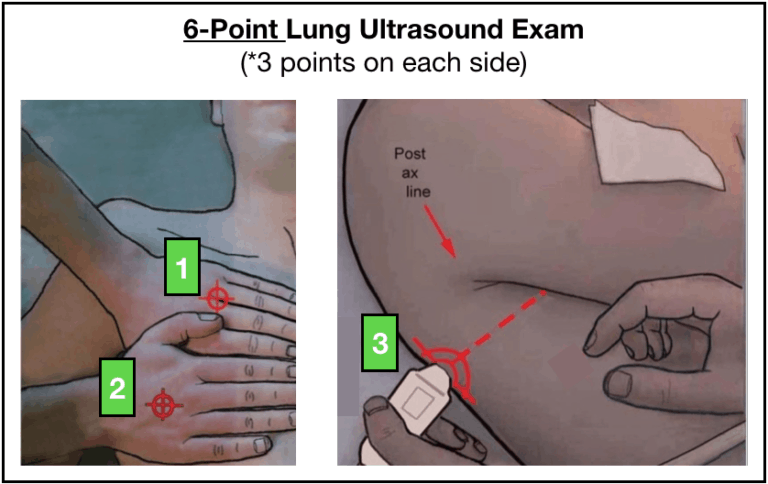
\includegraphics[width=0.5\linewidth]{images/us_protocols/6-points-protocol.png}
    \caption{6-points protocol (3 for each side) of BLUE}
    \label{fig:enter-label}
\end{figure}

Soldati et al. \cite{soldati2020proposal} presents a comprehensive framework aimed at optimizing the use of LUS in the diagnosis and management of COVID-19 employing a 12-points protocol. The authors highlight the  role of LUS as a diagnostic tool, expecially in the context of the COVID-19 pandemic as it is capable of detecting various lung conditions. Some of these are lung disease and acute respiratory distress syndrome, which are critical in managing COVID-19 pneumonia.
The authors pointed out the need for a unified approach, hence the team has developed a standardized protocol for its use in COVID-19 management.
This protocol includes specific recommendations regarding the equipment used, such as the adoption of wireless transducers and tablets.
These choices are made to minimize the risk of contamination during examinations, which is particularly important in the context of infectious diseases. 
By establishing a standardized method, the authors aim to ensure consistency in LUS practices across different healthcare settings.
 A significant contribution of the article is the introduction of a scoring system designed to classify the severity of lung involvement in COVID-19 patients based on LUS findings. This scoring system was developed through a collaborative effort involving the review of a substantial number of anonymized cases. By categorizing the severity of lung conditions, clinicians can make more informed decisions regarding patient management and treatment strategies, ultimately leading to better patient care.
The authors advocate for the establishment of an international database dedicated to sharing LUS images and videos to facilitate the collaboration among healthcare professionals and researchers worldwide. By pooling resources and knowledge, the medical community can enhance the development of pattern recognition algorithms and improve telemedicine capabilities. Such collaboration is crucial in a global health crisis, as it allows for the rapid dissemination of best practices and findings. The article provides practical guidelines for conducting LUS examinations effectively. Key recommendations include avoiding the use of cosmetic filters and specific imaging modalities that may obscure important findings. The authors stress the importance of achieving high frame rates during imaging to capture subtle lung changes accurately. Additionally, they recommend saving data in the Digital Imaging and Communications in Medicine (DICOM) format or as video files to ensure that visual findings can be reviewed comprehensively. With respect to the acquisition, 14 areas should be scanned per patient for 10 seconds. The areas are divided in this way:
\begin{itemize}
    \item 3 lateral
    \item 2 lateral
    \item 2 anterior
\end{itemize}.
The paper image to display the area of interest is illustrated in \autoref{fig:us_protocols:soldati_protocol}
To capture the largest surface area with a single scan, intercostal scans are required, thus an efficient and accurate way of detecting the ribs is crucial in the design of an autonomous ultrasound system. This thesis aims to face this problem using perception and human body modelling.
\begin{figure}[h]
    \centering
    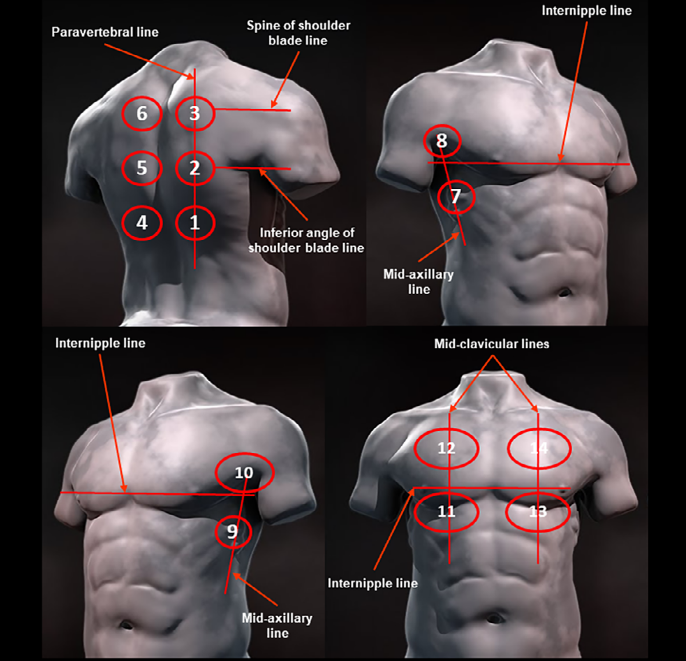
\includegraphics[width=0.5\linewidth]{images/us_protocols/14-points-protocol.png}
    \caption{The 14-points protocol proposed by Soldati et al.}
    \label{fig:us_protocols:soldati_protocol}
\end{figure}
      \newpage
\chapter{Framework Description}
\begin{figure}[t]
    \centering
    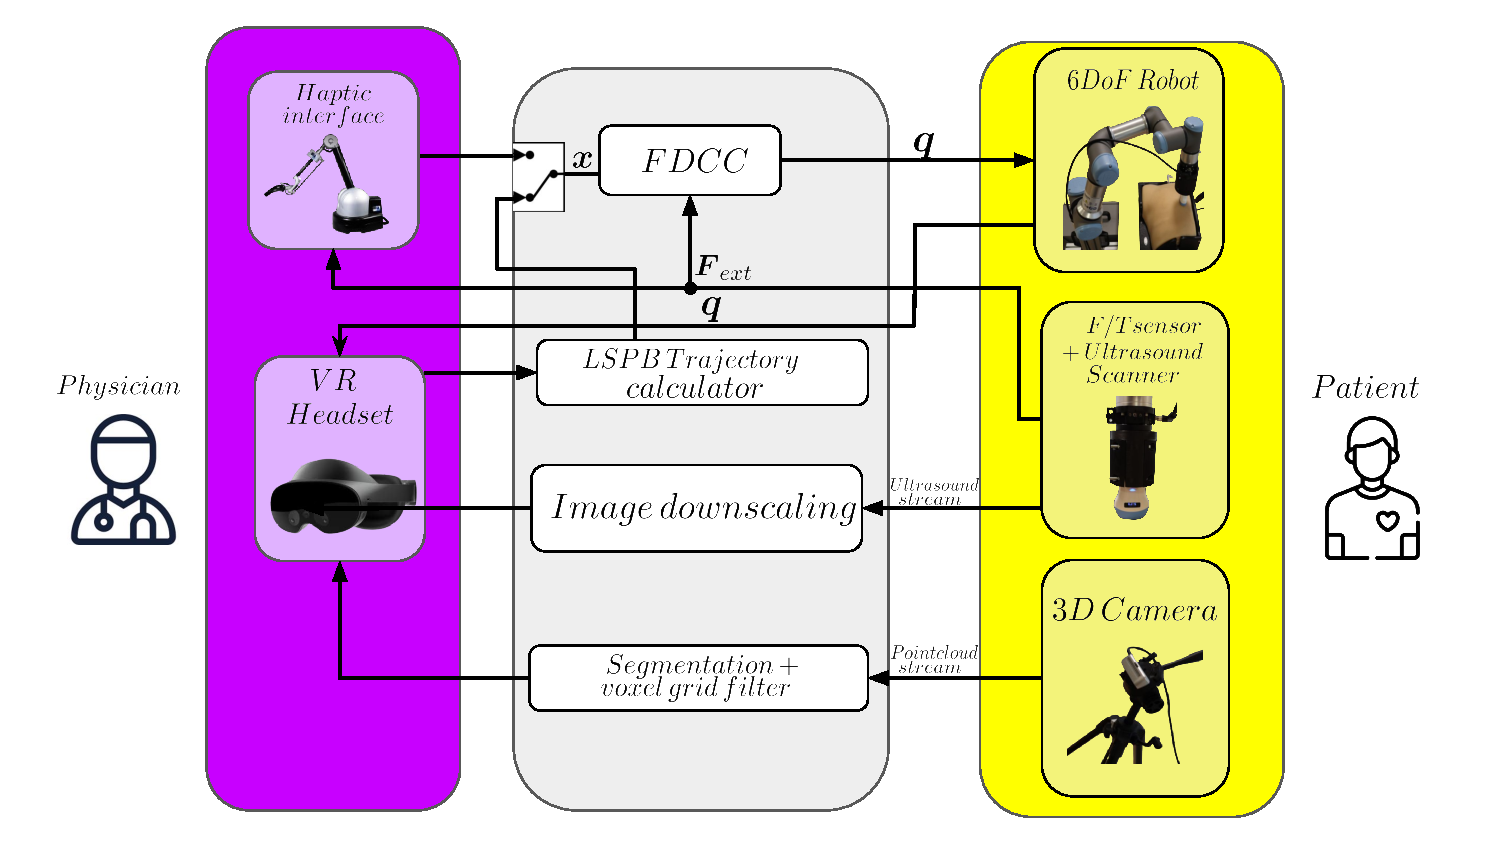
\includegraphics[width=1\columnwidth]{images/framework/framework.pdf}
    \caption{The proposed framework: the physician can teleoperate with the haptic interface or with the waypoint placing method. The visual signals coming from the sensors in the follower's setup are rendered into the VR headset while the force and wrenches feedback are used as input of haptic interface.} 
    \label{fig:framework}
\end{figure}

The remote robotised US framework consists of two main parts: the leader's side, which corresponds to the environment for the physician, and the follower's side, which corresponds to the environment for the patient (see \autoref{fig:framework}). The leader side profits from a real-time updated virtual reality scene streamed over a VR headset with the incoming feedback from the follower, such as the point cloud rendering of the patient overlapped to its SMPL model, the force and wrenches readings of the force and torque sensor mapped into the haptic interface, and the ultrasound probe stream, while the follower side capitalises on a 6Dof robot arm with a force and torque sensor that is controlled with a passive variable Cartesian impedance controller, an ultrasound probe and an RGB-D camera (see \autoref{fig:realenv}).

\subsection{Leader} 
% The leader part of this work is composed by three parts: the haptic interface, the virtual environment and the streaming of the output of the ultrasound probe. 
The haptic interface is the input device that the physician uses to control the relative position and orientation of the robot in real-time. It is controlled with a standard impedance control. We mapped the positions as follows:
\begin{equation}
\boldsymbol{P}^E_{des} = \boldsymbol{P}^E_{start} + \lambda(\boldsymbol{P}^H_{cur} - \boldsymbol{P}^H_{start})
\end{equation}
where $\boldsymbol{P}^E_{des}$ and $\boldsymbol{P}^E_{start}$ $\in \mathbb{R}^{m}$ are respectively the desired and starting position of the end effector, $\boldsymbol{P}^H_{cur}$ and $\boldsymbol{P}^H_{start}$ $\in \mathbb{R}^{m}$ are the current and starting position of the haptic interface, and $\lambda$ $\in \mathbb{R}^{m \times m}$ is a diagonal matrix scaling factor.
For the orientation representation, we used unit quaternions, which are well known to be computationally efficient and singularity-free. We implemented orientation mapping with unit quaternions in the following way:
\begin{equation}
\mathcal{Q}^H_{diff} = \overline{\mathcal{Q}}^H_{cur} * \mathcal{Q}^H_{start}
\end{equation}
\begin{equation}
\mathcal{Q}^E_{des} =\overline{\mathcal{Q}}^H_{diff} * \mathcal{Q}^E_{start}
\label{eq:q_des}
\end{equation}
where $\mathcal{Q}^H_{diff}\in \mathbb{R}^4$ is the relative orientation of the haptic interface with respect to its starting position, $\mathcal{Q}^H_{start}\in \mathbb{R}^4$ and $\overline{\mathcal{Q}}^H_{cur} \in \mathbb{R}^4$ are the starting and the conjugate of the current orientation of the haptic interface, $\mathcal{Q}^E_{des}\in \mathbb{R}^4$ is the desired orientation of the end effector, $\overline{\mathcal{Q}}^H_{diff}\in \mathbb{R}^4$ is the conjugate of $\mathcal{Q}^H_{diff}$ and  $\mathcal{Q}^E_{start}$ is the starting orientation of the end effector. The absence of the scaling factor in \eqref{eq:q_des} is motivated by the fact that we experienced a counterintuitive orientation control if we scale $\overline{\mathcal{Q}}^H_{diff}$.
%In this case, we avoided using a scaling factor because the rotation control seemed to become counterintuitive but it can be achieved anyway using the \verb|Slerp| function, which performs the spherical linear interpolation between quaternions and it is provided in many libraries such as Eigen. \\
At this point, a doctor would already be able to control the robot manipulator and receive force feedback from the patient, but he would miss the visual context of the operation. For this purpose, we recreated the room for ultrasonography in virtual reality (see  \autoref{fig:vrenv}), that can be explored through a VR headset.
We displayed the robot state by applying the joint values to a virtual model, which is visible to the physician. The point cloud computed from the RGBD sensor in the follower framework is rendered over the SMPL model, which is used just to monitor the patient pose. In our virtual scene, we also added a screen for broadcasting the ultrasound image. This feature can exploit VR capabilities to address the problem of not having the patient and the output of the ultrasonography in the same field of view since we can move the screen near the patient or make it follow the headset orientation in a dynamic way. This means that the physician will always be able to monitor both the patient and the ultrasound output, enhancing the control and safety of the teleoperation.
Another consequence related to the use of a virtual environment is the possibility for the doctor to move without limitations around the virtual patient, avoiding constraints on motion due to objects or the patient itself.

\begin{figure}[t]
    \centering
    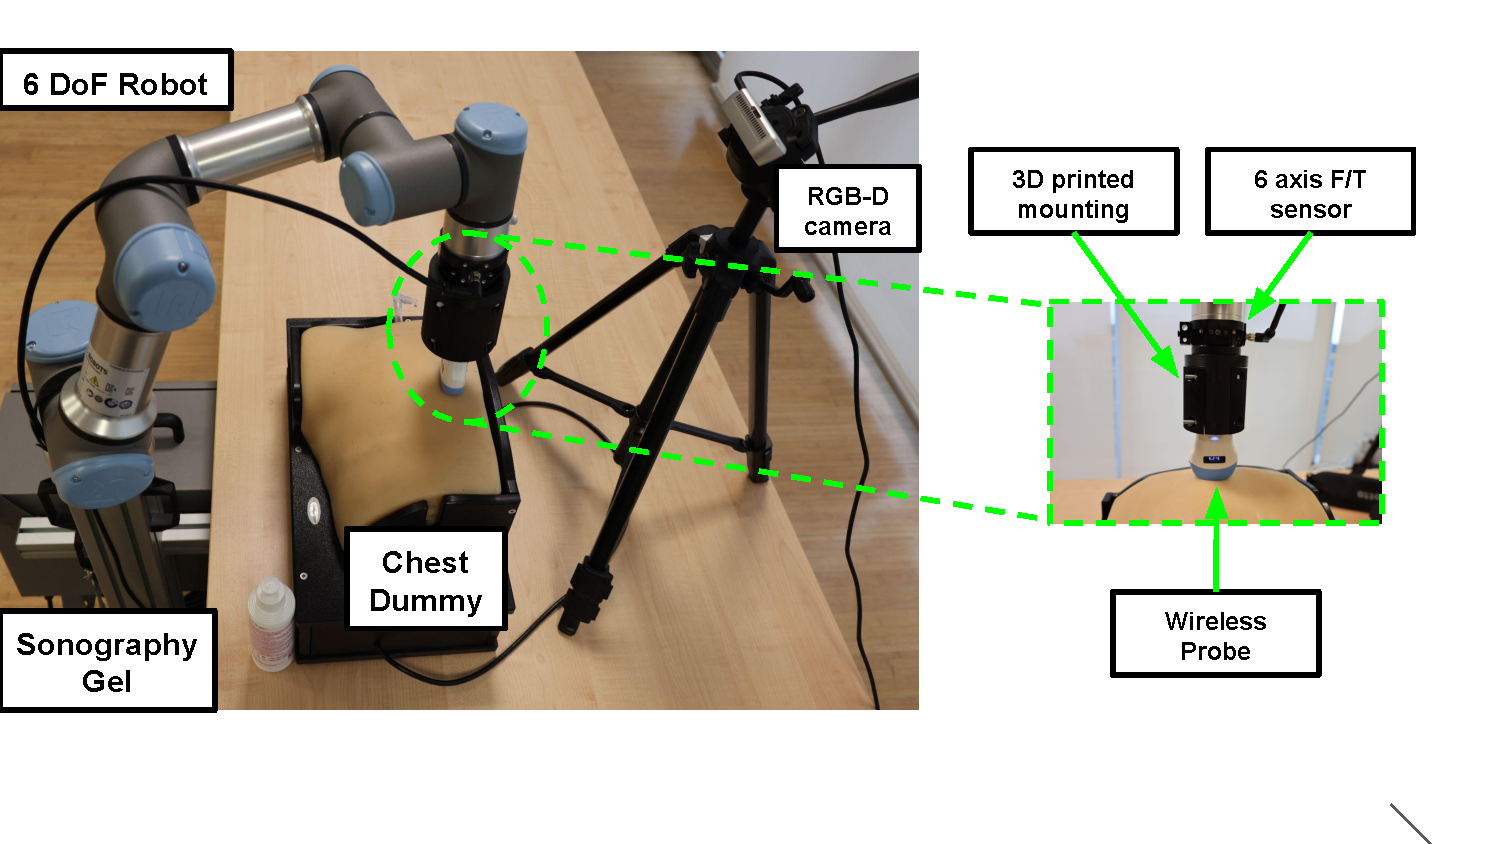
\includegraphics[clip,trim=0 50 0 20, width=1\columnwidth]{images/framework/setup.pdf}
    \caption{In the follower's setup, a chest dummy is used for the examination done by a robot manipulator equipped with a force/torque sensor and an ultrasound probe. A RGBD camera captures the 3d scene, creating a pointcloud.}
    \label{fig:realenv}
    % \vspace{-3mm}
\end{figure}


\begin{figure}[t]
    \centering
    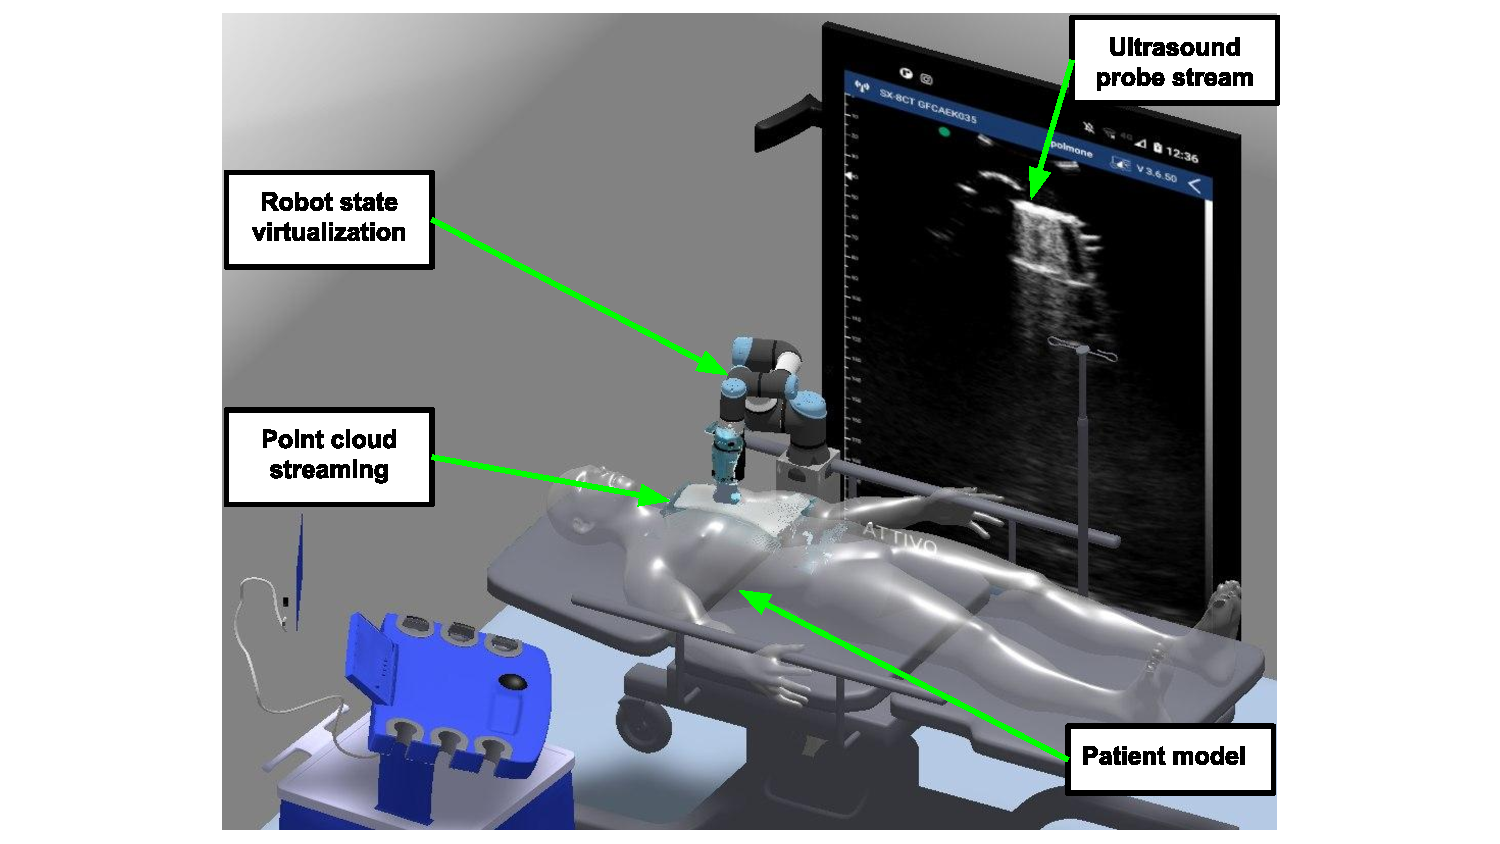
\includegraphics[width=0.9\columnwidth,trim={3.2cm 0 3.2cm 0},clip]{images/framework/env2.pdf}
    \caption{The virtual scene seen by the physician: the pointcloud of the chest dummy is mapped in the same relative pose of the patient's chest, and the stream of the ultrasound probe is put right in front of the physician's view as long as the robot is a digital twin.}
    \label{fig:vrenv}
    % \vspace{-3mm}
\end{figure}


%%%%%%%%%%%%%%%%%%%%%%%%%%%%%%%%%%%%%%%%%%%%
%%%%%%%%%%%%%%%%%%%%%%%%%%%%%%%%%%%%%%%%%%%%
\subsection{Follower}
For the robot's controller, we used the FDCC controller\cite{scherzinger2017forward}, where the closed-loop behaviour of a Cartesian compliant controller relates the external wrenches applied to the end-effector of the robot to a mass-spring-damper model as follows:
%is based on a mass-spring-damper model:
\begin{equation}
\boldsymbol{F}^{ext} = \boldsymbol{\Lambda}^d\ddot{\Tilde{\boldsymbol{x}}} + \boldsymbol{D}^d\dot{\Tilde{\boldsymbol{x}}} + \boldsymbol{K}^d\Tilde{\boldsymbol{x}},
    \label{eq:cartesian_impedance_inertia_shaping}
\end{equation}
where $\Tilde{\boldsymbol{x}} = \boldsymbol{x} - \boldsymbol{x}_d \in\mathbb{R}^{m}$ is the Cartesian error computed with respect to the desired Cartesian end-effector pose $\boldsymbol{x}_d$, $\boldsymbol{F}^{ext}\in\mathbb{R}^{m}$ is the external wrench applied on the end-effector, and $\boldsymbol{\Lambda}_d, \boldsymbol{D}_d ,\boldsymbol{K}_d\in\mathbb{R}^{m\times m}$ are the desired Cartesian inertia, damping, and stiffness, respectively. %The dynamics of this system is based on a mass-spring-damper model.

As system stability might be violated in the presence of a variable impedance controller, we enforced system passivity through the concept of passivity of the power port $\dot{\boldsymbol{x}}^T\boldsymbol{F}^{ext}$.
To do so, we introduce the formalism of port-Hamiltonian systems to describe the interaction model of the variable Cartesian impedance augmented with an energy tank~\cite{ferraguti2015energy} with dynamics:
\begin{equation}
    \dot{\textrm{x}}_t = \frac{\sigma}{\textrm{x}_t}\dot{\Tilde{\boldsymbol{x}}}^T\boldsymbol{D}^d\dot{\Tilde{\boldsymbol{x}}} - \frac{\boldsymbol{w}^T}{\textrm{x}_t}\dot{\Tilde{\boldsymbol{x}}},
\end{equation}
where $\textrm{x}_t \in \mathbb{R}$ is the state of the tank, $\sigma \in \{0,1\}$ modulates the energy storage, and $\boldsymbol{w}$ an the extra input of the port-Hamiltonian system defined as:
\begin{equation} \label{eq:variable_stiffness}
    \boldsymbol{w}(t) = \begin{cases} -\boldsymbol{K}^v(t)\Tilde{\boldsymbol{x}} & \mbox{if $T(\textrm{x}_t)>T_{min}$}  \\ 0 & \mbox{otherwise,} \end{cases}
\end{equation}
where $\boldsymbol{K}^v(t)$ is time-varying component of the stiffness
($\boldsymbol{K}^d(t) = \boldsymbol{K}^{min} + \boldsymbol{K}^v(t)$).
At each time instant, the tank's energy is defined by
$T(\textrm{x}_t)=\frac{1}{2}\textrm{x}_t^2$ and
$T_{min}\in\mathbb{R}^+$ is the minimum energy that the tank is
allowed to store. Thanks to~\eqref{eq:variable_stiffness}, we can
infer the condition $T(\textrm{x}_t)>T_{min}$ when the stiffness is
allowed to raise without violating the passivity constraint. However,
this bound does not prevent the energy of the tank to be drained
instantaneously, situation which leads to the complete loss of
performance. For this reason, it is reasonable to further constrain
the power flow of the tank when the energy is extracted from the tank
($\dot{T}(\textrm{x}_t) > - \eta \nonumber$), where
$\eta\in\mathbb{R}^+$ is the maximum allowed power.
The goal is to track a constant force $\boldsymbol{F}^d$ changing the stiffness matrix, which can be computed solving the QP in ~\eqref{eq:general_QP_formulation}. The optimisation problem involves a trade-off between the precise tracking of a desired wrench and the necessity to uphold a limited level of stiffness.
Inspired by~\cite{zhao2022hybrid}, we formulated the QP as follows:
\begin{align}
    \min_{\substack{\boldsymbol{K}^d \in \mathbb{R}^{m \times m} }} \: & \frac{1}{2} \left( \| \boldsymbol{F}^{ext} - \boldsymbol{F}^{d} \|_{\boldsymbol{Q}}^2 + \| \boldsymbol{K}^{d} - \boldsymbol{K}^{min} \|_{\boldsymbol{R}}^2 \right) \nonumber \\ 
    \quad  \text{s.t.   } \boldsymbol{K}^{min} &\le \boldsymbol{K}^d \le \boldsymbol{K}^{max} \nonumber \\
    \boldsymbol{F}^{min} &\le \boldsymbol{F}^{ext} \le \boldsymbol{F}^{max} \label{eq:general_QP_formulation} \\
    - \boldsymbol{K}^d \Tilde{x} &\leq \sigma \dot{\Tilde{\boldsymbol{x}}}^T \boldsymbol{D}^d \dot{\Tilde{\boldsymbol{x}}} - \Tilde{\boldsymbol{x}}^T 
    \boldsymbol{K}_{min} \dot{\Tilde{x}} + \frac{ T_{t-1} - T_{min}}{\Delta t} \nonumber \\
     %& T(\textrm{x}_t) \ge T_{min} \nonumber \\
    - \boldsymbol{K}^d \Tilde{x} &\leq \sigma \dot{\Tilde{\boldsymbol{x}}}^T \boldsymbol{D}^d \dot{\Tilde{\boldsymbol{x}}} - \Tilde{\boldsymbol{x}}^T 
    \boldsymbol{K}_{min} \dot{\Tilde{x}} - \eta \nonumber
   % & \dot{T}(\textrm{x}_t) \ge - \eta \nonumber
\end{align}
where $N$ is the length of the time window, $\boldsymbol{Q}$ and $\boldsymbol{R}$ $\in \mathbb{R}^{m\times m}$ are diagonal positive definite weighting matrices, $\boldsymbol{K}^d \in \mathbb{R}^{m\times m}$ is the desired stiffness of the Cartesian impedance controller, $\boldsymbol{K}^{min}$ and $\boldsymbol{K}^{max}$ $\in \mathbb{R}^{m\times m}$ are respectively the minimum and maximum allowed stiffness, $\boldsymbol{F}^{ext} \in \mathbb{R}^{m}$ is the wrench of the impedance interaction model, which can be modelled with \eqref{eq:cartesian_impedance_inertia_shaping}, $\boldsymbol{F}^d \in \mathbb{R}^{m}$ is the desired interaction wrench and $\boldsymbol{F}^{max}/\boldsymbol{F}^{min} \in \mathbb{R}^{m}$ is the maximum/minimum wrench that the robot can exert. %The constraint inequality between vectors is element-wise.
The last two constraints limit the maximum energy $T_{min}$ which can be injected in the system and the rate $\eta$ at which the energy is injected and are obtained from $T \le T_{min}$ and $\dot{T} \le -\eta$. 
$1/\Delta t$ is the controller frequency. 
When $T \le T_{min}$ is not satisfied, the stiffness decreases to its minimum ($\boldsymbol{K}^d = \boldsymbol{K}^{min}$). 


More details on the QP problem formulation and energy tank constraint definition are available in~\cite{beber2023passive} referring to the VF-CF control law, but assuming the target force fixed to be fixed instead of pre-computed.
The measured force and torque are used for control but also as feedback for the physician through the haptic interface. A straight one-to-one mapping of these quantities from the sensor to the device produces some vibrations on the haptic interface. This is related to the noise in the F/T sensor readings. To address this problem, we added an exponential moving average filter (EWMA) \cite{roberts1959}, which represent a good trade-off between smoothness and introduced delay:
\begin{equation}
    \boldsymbol{F}^{ext}_H = \boldsymbol{\alpha} \boldsymbol{F}^{ext}_{cur} + (\boldsymbol{I} - \boldsymbol{\alpha}) \boldsymbol{F}^{ext}_{old} 
\end{equation}
where $\boldsymbol{F}^{ext}_H \in \mathbb{R}^{m}$ is a vector of forces and torques that are the target output of the haptic device, $\boldsymbol{F}^{ext}_{cur}$ and $\boldsymbol{F}^{ext}_{old} \in \mathbb{R}^{m}$ are the vectors of forces and torques of the current and precedent control loop, $\boldsymbol{I} \in \mathbb{R}^{m \times m}$ is the identity matrix, and $\boldsymbol{\alpha} \in \mathbb{R}^{m \times m}$ is a diagonal matrix of weights.
 


  

      \input{sections/network_setup}
      \newpage
\chapter{Connection requirements}

The problem of transmitting large data is one of the open problems in the information technology research area. A teleoperated system like the one presented in this work need a stable, low-latency connection with high bandwidth requirements. In the proposed framework I needed to transmit different types of data with different requirements. We defined requirements as \textit{critical} when a connection drop could harm the patient or cause damage to the equipment.
%\begin{itemize}
%	\item Ultrasound image stream: high bandwidth with medium latency
%	\item Force/Torque measurement from the F/T sensor: very low bandwidth but also very low latency
%	\item Point cloud of the patient: high bandwidth with medium latency
%	\item leader haptic device target pose: very low bandwidth and very low latency
%	\item SMPL body parameters: very low bandwidth and medium latency
%	content...
%\end{itemize}
\newcommand{\cmark}{\ding{51}}%
\newcommand{\xmark}{\ding{55}}%

\begin{table*}[!ht]
	\centering

	\begin{tabular}{|c|c|c|c|}
		\hline
		& Critical & High Bandwidth($>$5MB/s) & Low Latency ($<$5ms)\\
		\hline
		Ultrasound image stream & \xmark & \cmark & \cmark \\
		\hline
		Force/Torque measurement & \cmark & \xmark & \cmark \\
		\hline
		Haptic device pose measurement & \cmark & \xmark & \cmark \\
		\hline
		Point cloud of the patient & \xmark & \cmark & \xmark \\
		\hline
		SMPL body parameters  & \xmark & \xmark & \cmark \\
		\hline
		Robot state & \xmark & \xmark & \cmark \\
		\hline
	\end{tabular}
	\caption{Connection requirements for the teleoperation framework}
	\label{tab:comparison}
\end{table*}

      \chapter{Human Body Estimation}
In this chapter, I will explain how I managed to estimate the parametric model of the patient exploiting visual information.

\section{SMPL models family}
For the body shape and pose, there is a well known model called SMPL (Skinned Multi-Person Linear Model) \cite{SMPL:2015} which is a realistic 3D model of the human body that is based on skinning and blend shapes. SMPL is learned from thousands of 3D body scans. SMPL model pose is described by 23 body joints together with body position and orientation called $\vec{\theta}$, while the body shape is described by 10 parameters called $\vec{\beta}$. Each $\theta_i, i \in [1,21] $ represents the 3D orientation of a human joint with respect to its kinematic parent. The kinematic tree is expressed as a connectivity map that connect each joint to its child, as shown in \autoref{fig:human-body-estimation:kin_tree}.
\begin{figure}[h]
    \centering
    
\includegraphics[width=0.07\linewidth]{images/kinematic_tree.png}
    \caption{The SMPL kinematic tree}
    \label{fig:human-body-estimation:kin_tree}
\end{figure}
Orientations are represented by rotation vectors and can be converted to rotation matrices using the Rodriguez formula. % The inference of the SMPL is the prediction of the joint location thanks to a joint regressor, then the computation of the blend skinning of the model starting from the T-pose and finelly the .%
Since the model is linear, the inference time is fast.
There exist multiple variants of this model:
\begin{itemize}
    \item SMPL-H\cite{MANO:SIGGRAPHASIA:2017} is the extended version of SMPL that accounts also for hands position. It leverages on 21 body joints from the SMPL model, replacing the two additional joints related to the hand position with 15 additional joints for each hand.
    \item SMPLX\cite{SMPL-X:2019} (SMPL eXpressive) is the extended version of SMPL-H which accounts also for the face expressions. The total number of joints is 54 which includes joints for the neck, jaw, eyeballs, and fingers. 
\end{itemize}
The difference between SMPL and SMPLX is show in \autoref{fig:human-body-estimation:smpl}.
\begin{figure}[h]
    \centering
    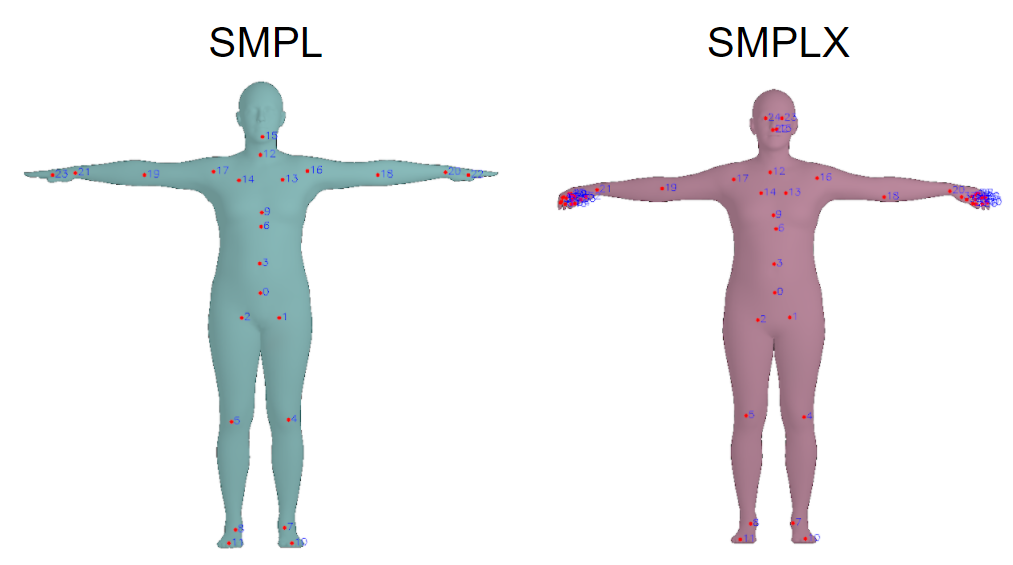
\includegraphics[width=0.7\linewidth]{images/smpl.png}
    \caption{The comparison of the number and location of joints for SMPL and SMPLX}
    \label{fig:human-body-estimation:smpl}
\end{figure}
These more recent extensions of SMPL can be used in tasks where knowing the exact hand configuration is crucial or when the facial expression information can be exploited in some way. In my opinion, SMPL-H and SMPLX will be soon introduced in different human-robot collaboration scenarios. Since for RLU hands and facial expressions were not included in the logic of my thesis I took the SMPL for modelling the patient state.

\section{Human body pose estimation}
As already mentioned in the previous section, the SMPL model is composed by $\vec{\theta}$ and $\vec{\beta}$. It is possible to animate a SMPL model in real-time if $\vec{\beta}$ does not need to be optimized, updating just the $\vec{\theta}$ parameters of the model.
For this purpose I used a \verb|ZED2| stereo camera which integrates an AI body tracking module\cite{zed_body_tracking} based on the depth and RGB image measured by the sensor itself. The body tracking module provides different skeleton models. I chose the one more similar to SMPL, which is also the most informative, since it is the one with the highest number of keypoints (38). A figure showing the pose of the keypoints is reported in \autoref{fig:human-body-estimation:zed_kp}.
\begin{figure}[H]
    \centering
    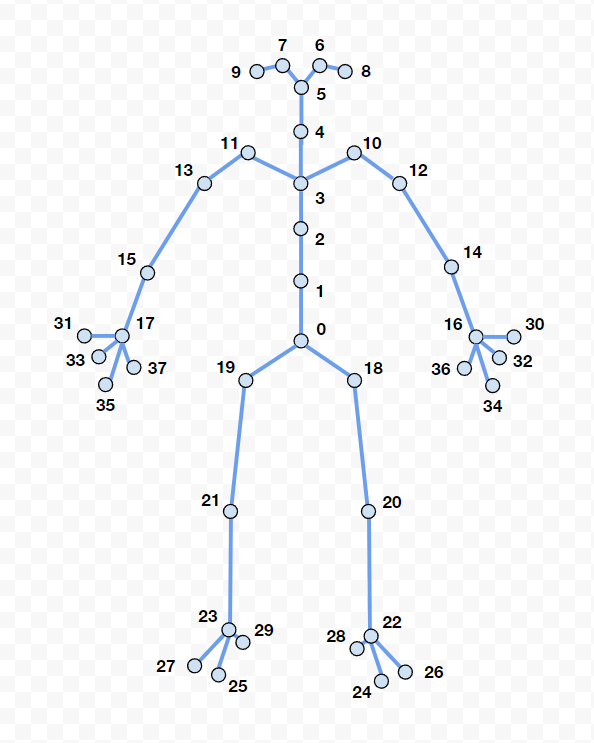
\includegraphics[width=0.5\linewidth]{images/zed_kp.png}
    \caption{BODY38 model provided by the ZED SDK}
    \label{fig:human-body-estimation:zed_kp}
\end{figure}
Comparing \autoref{fig:human-body-estimation:smpl} and \autoref{fig:human-body-estimation:zed_kp} it is easy to notice that the joint location is similar between the two models, so it was straight forward to compute the right input for the SMPL model for the real time animation. Since the \verb|ZED| AI module already provides the local orientation of each joints with respect to its parent in the kinematic tree (which is the same of the SMPL), it was sufficient to convert from the quaternion notation for the orientation to the rotation vector notation.

\section{Human body shape estimation}
\label{section:human-body-shape-estimation}
Given that this master's thesis aims to address the problem of the physical variability between patients in RLU, $\vec{\beta} \in \mathbb{R}^{10}$ is a crucial parameter to be considered since it affects the rib cage dimension and position. An external source of information is required in order to evaluate a metric for the shape parameters optimization. I decided to use the same exteroceptive sensor used for the pose estimation procedure: the \verb|ZED2|. Therefore, I retrieved the raw point cloud of the scene. 

\section{Human Instance Segmentation with YOLOv8}
Since I needed an intelligent way of ignoring points not belonging to the human, I exploited YOLOv8 segmentation neural network from Ultralytics in order to detect which image pixel belongs to the patient. YOLOv8 segmentation is an advanced computer vision model that combines object detection with instance segmentation. Ultralytics provides different models for the instance segmentation of 80 different classes. 
When applied to human body segmentation, it not only identifies humans in an image but also generates a precise mask outlining the shape and boundaries of the body. This is achieved through pixel-level predictions, allowing the model to differentiate the human body from the background and other objects. YOLOv8's segmentation capabilities are highly efficient, making it suitable for real-time applications like pose estimation, augmented reality, and medical imaging.  

\section{Point Cloud Filtering using YOLOv8Seg Mask}
The mask computed by YOLO is represented by the vertices of a polygon. I converted it to a bit mask matrix through the \verb|fillPoly| of \verb|opencv| having 1 or 0 for each pixel of the original image. The resulting image is then used to decide which points of the point cloud to discard. Moreover, I exploited the bounding box provided by YOLO in addition to the mask to limit the amount of computation needed to filter the point cloud. To be more explicit, I restricted the double nested loop over the image pixels to the bounding box instead of the full image. The resulting point cloud is illustrated in \autoref{fig:human-body-estimation:yolo-seg}


\begin{figure}[h]
    \centering
    \subfloat[\centering RGB Image from the left sensor of the stereo camera with the yolo segmentation mask colored in red]{{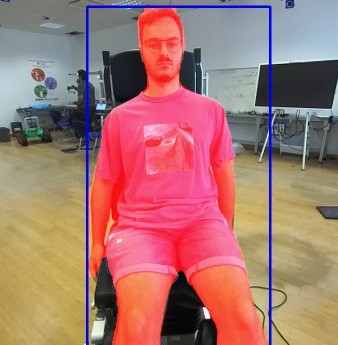
\includegraphics[width=5cm]{images/body_estimation/yolo_seg.jpg} }}%
    \qquad
    \subfloat[\centering Point cloud obtained removing the points relative to the pixels filtered by the mask]{{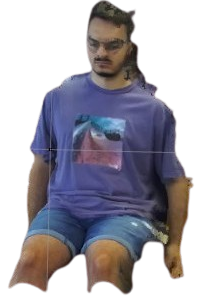
\includegraphics[width=3cm]{images/body_estimation/point_cloud.png} }}%
    \caption{}%
    \label{fig:human-body-estimation:yolo-seg}%
\end{figure}

\section{SKEL, a biomechanical model}
SKEL\cite{keller2023skel} is a biomechanical skeleton model that maps the SMPL skinned model to its anatomical skeleton. The new model differs from the existing SMPL model in several key ways:
\begin{itemize}
    \item Anatomical accuracy: In comparison to SMPL, SKEL offers more precise joint placements and anatomically correct bone orientations. It includes biomechanical factors, like better knee alignment and arm supination, that enable a more accurate depiction of human anatomy.
    \item Posture parameters: SKEL is more effective in regressing precise anatomical joints from video data because it has fewer posture parameters (46), as opposed to SMPL's (72). Applications in computer vision and biomechanics benefit from this reduction in parameters.
    \item Biomechanical features: SKEL incorporates a biomechanical shoulder blade that enables for more realistic movement in place of the SMPL's approximation shoulder structure. Additionally, it simulates how the ulna and radius bones move in the forearm pronation and supination, which constitute a major advancement above the SMPL's basic rotation around the elbow.
    \item Integration of skin and skeleton: SKEL enables direct animation of both components by concurrently rigging the skin and skeleton meshes with the same pose parameters. For this reason, SKEL can inherit the pose and shape directly from SMPL.
    \item Data utilization: To improve the accuracy of the skeletal structure and joint placements, SKEL makes use of the BioAMASS dataset, which integrates motion capture data with anatomical information. In comparison, SMPL does not include such comprehensive biomechanical data.
\end{itemize}

Compared to the SMPL framework, SKEL represents a substantial leap in producing 3D human models that are more lifelike and anatomically precise. An illustrative image of SKEL can be observed in \autoref{fig:human-body-estimation:skel} 
\begin{figure}[H]
    \centering   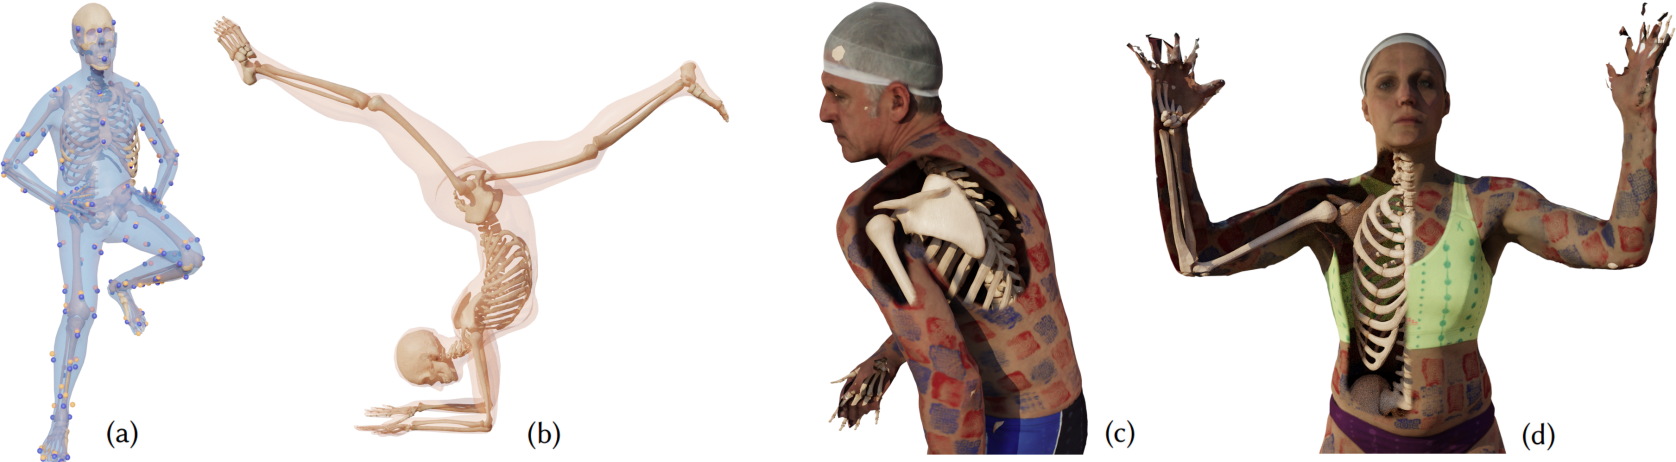
\includegraphics[width=0.7\linewidth]{images/skel.png}
    \caption{An image taken from the SKEL paper, as we can see in the images on the left, both the skin and the skeleton are present in the output of the SKEL model}
    \label{fig:human-body-estimation:skel}
\end{figure}
\section{SKEL Fitting from SMPL}
Since I computed the SMPL from the patient state in \autoref{section:human-body-shape-estimation}, the next step was to compute the skeleton inside the SMPL mesh. Since SKEL has the same surface mesh topology and shape parameters $\vec{\beta}$ as SMPL, it can be directly fit to existing SMPL meshes by optimizing its pose parameters to minimize the vertex-to-vertex
error between the SMPL skin and the SKEL skin. The alignment is avoid local minima by aligning the model in this order:
\begin{enumerate}
\item Align pelvis
\item Align forearm and thighs
\item Align elbows and knees 
\item Align hands, feet, and neck
\end{enumerate}
The order is the same of the kinematic tree since each joint position depends on its predecessor. In order to locally optimize some particular joints, it is sufficient to mask the not relevant contributions in the loss computation. The loss used for the optimization were:
\begin{itemize}
    \item Pose loss: The loss between the joint position of SMPL and the one of SKEL
    \item Vertex loss: Since the skin mesh of SMPL is the same as SKEL, it is possible to compute vertex-wise displacement
    \item Scapula loss: loss added to regularize the scapula fitting avoiding large values, implemented with masking on non-relevant joints
    \item Spine loss: loss added to regularize the spine fitting avoiding large values, implemented with masking on non-relevant joints
\end{itemize}
\TODO add formula
\section{Modelling the rib cage projection on the skin}
Once the SKEL model is computed from the SMPL retrieved from the point cloud, we need to understand where it is located during the robot interaction with the skin. Different geometrical intuition and approximation can be used to estimate how the rib cage is projected on the skin. My first idea was to radially project the skeleton mesh vertices to the skin. The result was poor, especially for ribs far from the projection centre. I then switched to cylindrical projection, considering the cylinder axis parallel to the backbone. The results were qualitatively more realistic than the one produced by the spherical projection. The projection was implemented using ray casting algorithm provided by \verb|Open3d| that finds the 3D intersection point of a ray to a mesh. A visual comparison between radial and cylindrical projection is shown in \autoref{fig:human-body-estimation:skeleton-projection}.
\begin{figure}[H]
     \centering
     \begin{subfigure}[b]{0.3\textwidth}
         \centering
        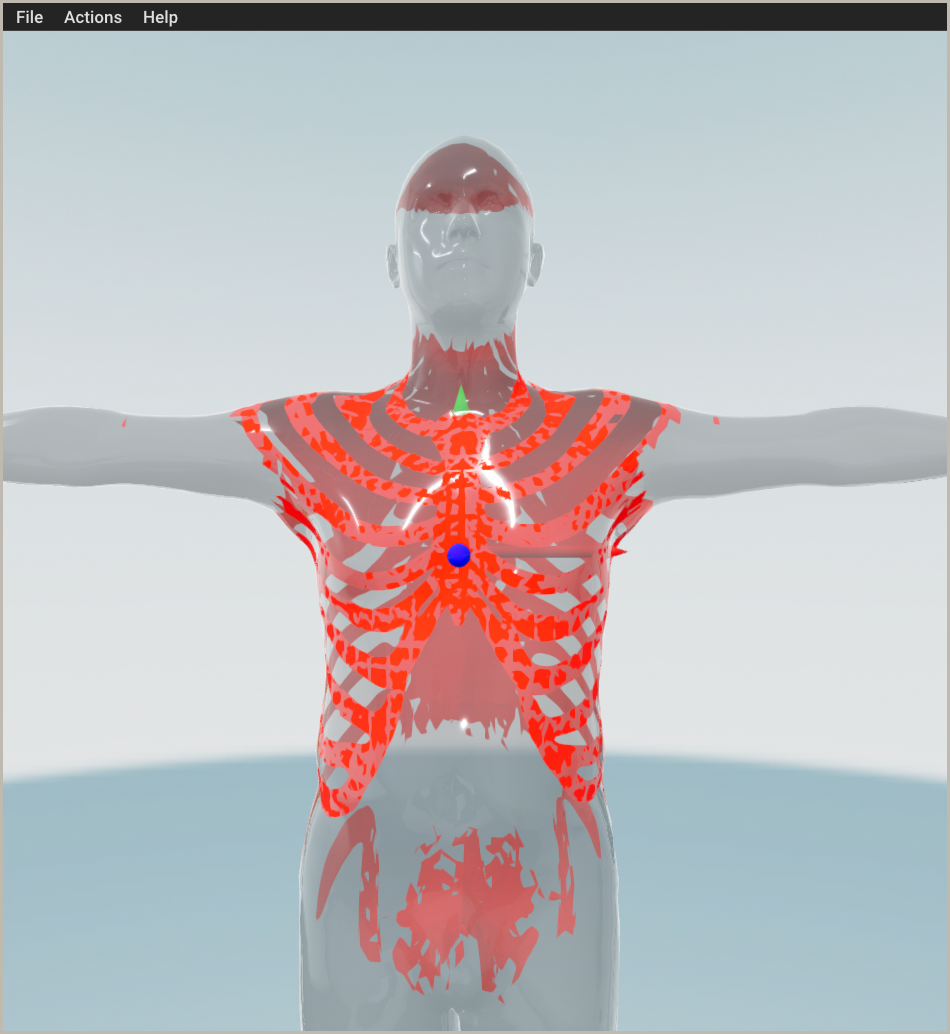
\includegraphics[width=\textwidth]{images/body_estimation/radially_proj.png}
         \caption{}
         \label{}
     \end{subfigure}
     \hfill
     \begin{subfigure}[b]{0.3\textwidth}
         \centering
         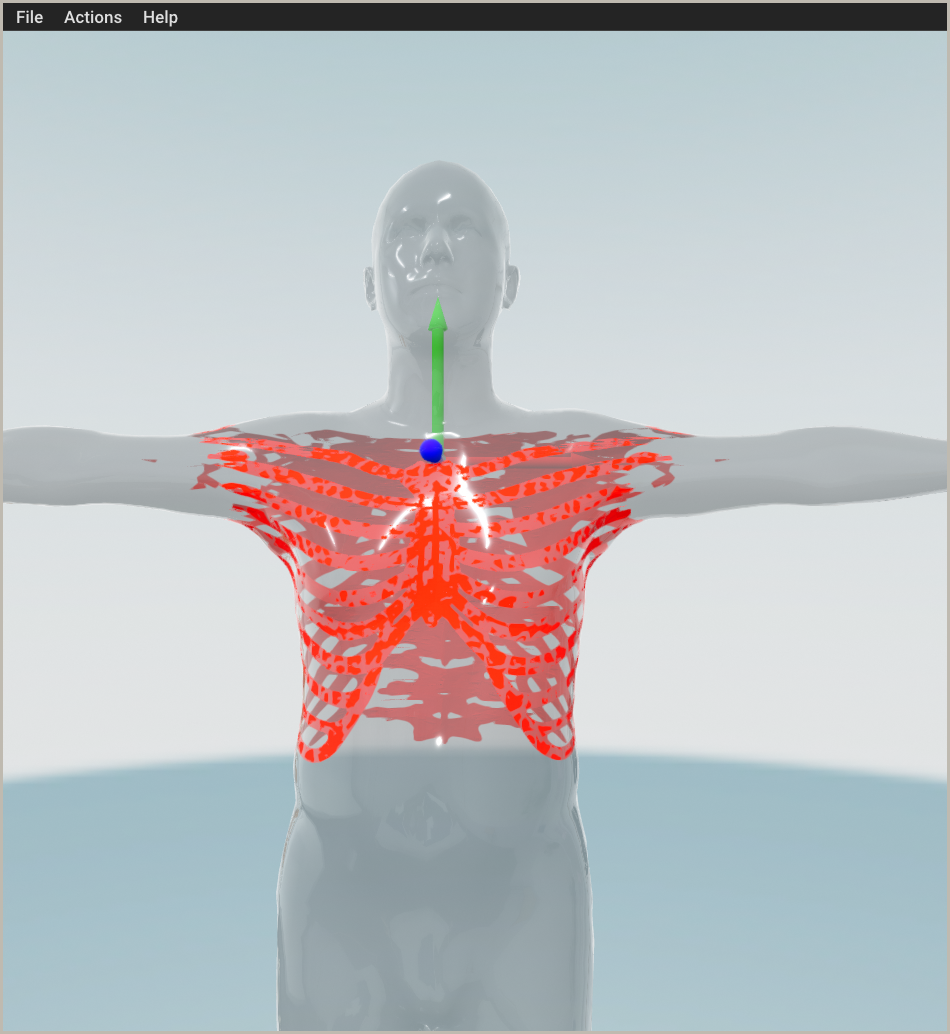
\includegraphics[width=\textwidth]{images/body_estimation/cylindrical_proj.png}
         \caption{}
         \label{}
     \end{subfigure}
\caption{Comparison between the two projection methods tested: on the left the radial projection, on the right the cylindrical projection}
\label{fig:human-body-estimation:skeleton-projection}
\end{figure}

Since each vertex is projected on the skin, the result is a point cloud. We can reconstruct a mesh from the projection connecting each vertex to his adjacent vertices in the original rib cage mesh.
The result of such operation is shown in \autoref{fig:human-body-estimation:projection_reconstruction}. As we can notice, the ribs are reconstructed correctly.
%% TODO parlare dell'ottimizzazione con loss functions ecc
\begin{figure}[H]
    \centering   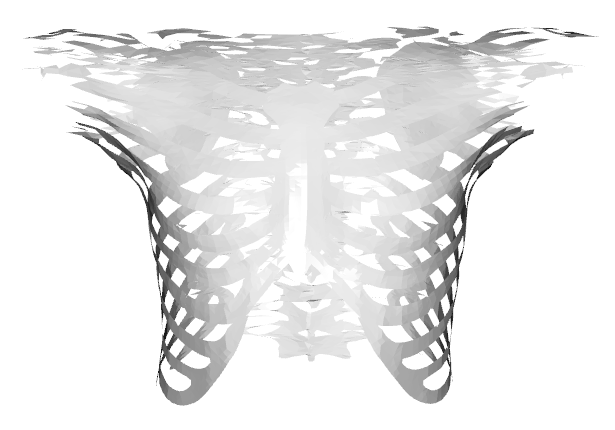
\includegraphics[width=0.7\linewidth]{images/body_estimation/rib_cage_proj.png}
    \caption{The resultant mesh obtained from the point cloud retrieved by the cylindrical projection of the rib cage original mesh.}
    \label{fig:human-body-estimation:projection_reconstruction}
\end{figure}
The idea is to create a virtual fixture that guide the physician towards the intercostal area, exploiting the semantic knowledge expressed by the SKEL model to compensate the lacks of the teleoperation.
      \newpage
\chapter{Virtual Fixtures}

Virtual fixtures (VF), also called active constraints, are a family of algorithms used for limiting the workspace of the robot for safety and accuracy reasons, thus they are widely used in medical robotics. They were introduced in 1992~\cite{rosemberg1992use} by Rosemberg in an augmented reality teleoperation setup to simulate physical barriers, fields, and guides, designed to assist in the user during the teleoperation. 
VFs can be modelled with different shapes as shown in~\cite{bettini2004vision}where the author proposed a tube-like boundary with an admittance control and haptic feedback. Later on, different works show the crucial importance of VFs in medical robotics scenarios where the workspace of the robot must be limited to the area of interest to avoid hurting patients. In 2012 Rydén et al.~\cite{ryden2012forbidden} proposed an algorithm for the identification of a forbidden region virtual fixture from point clouds analysis that was used for operating on a beating hearth. The virtual fixture region is computed, considering each point of the point cloud as a 3D sphere with a particular radius. A known problem of VFs is the non passivity of the system when crossing or getting closer to the boundaries. 

\section{Classification of VFs}

A good classification of these algorithms is given in~\cite{bowyer2014active}. One of the most significant classifications is whether the fixture belongs to the \textit{forbidden region VF} or \textit{guidance VF}. The former bounds a manipulator’s tool to certain regions within its task or joint space, the latter encourages the user to move the tool along a specific pathway or toward a specific target. Usually, guidance constraints are more intrusive upon the user than forbidden region constraints in normal operation. The second meaningful classification for this work highlighted by the author is whether the constraint is \textit{unilateral} or \textit{bilateral}.
A unilateral virtual fixture is a constraint active only by one side, while the bilateral acts on both sides. 
Regional VFs (forbidden region) often are implemented with unilateral constraints, whereas guidance VFs leverage on bilateral limits.
The last distinction is between \textit{static} and \textit{dynamic} constraints that depend on if the geometry exploited by the algorithm change during the operation.

\section{VFs Generation}
In the literature, different methods for the generation of virtual fixture were proposed. The survey~\cite{bowyer2014active} mentions the most common types of constraint representations used in the literature.
\begin{enumerate}
    \item (a) Point: A single 3d point can be used to generate an attractive or repulsive potential field
    \item (b) Line: can be used to generate a guidance
    \item (c) Parametric curve: generalization of the line for task that requires some dexterity
    \item (d) Plane: Usually used as a forbidden region constraint to limit the robot workspace
    \item (e) Parametric surface: generalization of the plane. A well-known way for generating a parametric surface from a set of points is the Non Uniform Rational Basis-Splines (NURBS)
    \item (f) Polygonal Mesh: Non-parametric but realistic way of representing a real object. Can be used when the fidelity of the constraint is crucial for the task.
    \item (g) Point Cloud: A virtual fixture can be generated by a point cloud as explained in~\cite{ryden2012forbidden} 
    \item (h) Volumetric primitives: Boolean algebra can be applied to 3d mesh to obtain complex shapes maintaining computation efficiency in order to model situations in which the efficiency is critical
    \item (i) Explicitly described areas: work well in small scale scenarios but suffer from the curse of dimensionality.
\end{enumerate}
\begin{figure}[H]
    \centering   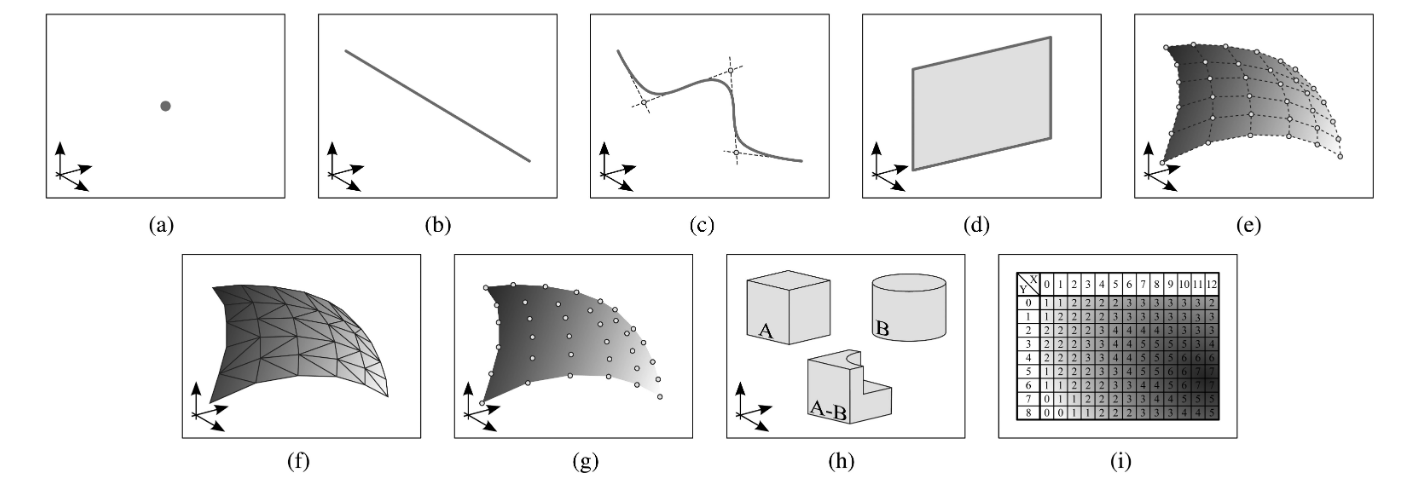
\includegraphics[width=0.7\linewidth]{images/virtual_fixtures/vf_geoms.png}
    \caption{The most common types of virtual fixture geometries reported by Bowyer et al.}
    \label{fig:virtual_fixture:vf_geoms}
\end{figure}
\TODO storia delle VF con reference
\cite{selvaggio2018passive}
\cite{soldati_proposal_2020}
      
    \endgroup


    % bibliography - bibtex format
    %
    % add chapter to index
    \addcontentsline{toc}{chapter}{Bibliography}
    % alphabetical order of authors
    \bibliographystyle{plain}
\bibliography{bibliography/lung_us,bibliography/smpl, bibliography/virtual_fixture, bibliography/reference_med, bibliography/reference_vic,bibliography/reference_vr}
%%%%%%%%%%%%%%%%%%%%%%%%%%%%%%%%%%%%%%%%%%%%%%%%%%%%%%%%%%%%%%%%%%%%%%%%%%
%%%%%%%%%%%%%%%%%%%%%%%%%%%%%%%%%%%%%%%%%%%%%%%%%%%%%%%%%%%%%%%%%%%%%%%%%%
%% Nota
%%%%%%%%%%%%%%%%%%%%%%%%%%%%%%%%%%%%%%%%%%%%%%%%%%%%%%%%%%%%%%%%%%%%%%%%%%
%% In the bibliography, all the sources consulted for the dissertation 
%% have to be cited and listed in alphabetical order by the 
%% first author's surname.
%%
%% According to the source material, the quotation has to be as follows:
%%
%% BOOKS
%% Surname and initial/s of the name/s of the author/s, date of edition,
%% publishing house and (if applicable) number of edition.
%% 
%% JOURNAL ARTICLES 
%% Surname and initial/s of the first name/s of the author/s,
%% title of the article, name of the journal, volume number, issue number
%% and page numbers.
%% 
%% CONFERENCE PAPERS
%% Surname and initial/s of the name/s of the author/s,
%% year of the conference, title of the article, name of the conference,
%% place of the conference, conference dates, page numbers.
%% 
%% CITING WEB RESOURCES
%% The consulted webpages have to be listed in alphabetical order. 
%% It is necessary to:
%%   - Copy the specific URL (the web address) of the consulted webpage
%%   - If available, indicate the surname and first name of the author/s,
%%     the title and subtitle of the text
%%   - If available, indicate the last date you retrieved the webpage
%%     (day/month/year).   
%%%%%%%%%%%%%%%%%%%%%%%%%%%%%%%%%%%%%%%%%%%%%%%%%%%%%%%%%%%%%%%%%%%%%%%%%%
%%%%%%%%%%%%%%%%%%%%%%%%%%%%%%%%%%%%%%%%%%%%%%%%%%%%%%%%%%%%%%%%%%%%%%%%%%
    

    \titleformat{\chapter}
        {\normalfont\Huge\bfseries}{Appendix \thechapter}{1em}{}
    % Appendix / attachment section - optional
    \appendix
    \chapter{Title first appendix}


\end{document}
